\documentclass[12pt]{article}
\usepackage[utf8]{inputenc}
\usepackage[russian]{babel}
\usepackage{amsmath}
\usepackage{amsthm}
\usepackage{hyperref}
\usepackage{xcolor}
\usepackage{graphicx}
\usepackage{subcaption}

\renewcommand{\baselinestretch}{1.} 
\renewcommand{\familydefault}{\sfdefault}

\begin{document}
\title{Компьютерная лингвистика и анализ текста. ДЗ №1}
\author{О. Р. Дон}
\maketitle

\section*{Лексико-статистический анализ двух текстов на русском языке}

В качестве материалов для анализа были использованы тексты:
\begin{itemize}
\item[1.] литературный -- глава 2 из книги Л. Кэрролла "Алиса в стране чудес";
\item[2.] научно-технический -- статья Ивашко Кристины Сергеевны "Медиатекст как система представления информации" (\href{http://sci-article.ru/stat.php?i=1579679587}{ссылка}).
\end{itemize}

\subsection*{Использованные инструменты}

Для проведения лексико-статистического анализа были использованы:
\begin{itemize}
\item[1.] Python 3.6, Jupyter notebook (сама тетрадь и список зависимостей приложены в отдельном архиве);
\item[2.] библиотека для обработки текстов NLTK (\href{https://www.nltk.org/}{ссылка});
\item[3.] морфологический анализатор Yandex MyStem (\href{https://yandex.ru/dev/mystem/}{ссылка}) и обертка для Python PyMyStem3 (\href{https://github.com/nlpub/pymystem3}{ссылка}).
\end{itemize}

\subsection*{Полученные лексико-статистические данные}

Морфологический анализатор MyStem умеет разбивать текст на предложения и благодаря этому можно получить данные о длинах предложений. Рассчет общестатистических данных проводился путем обычного подсчета элементов. Так же был составлен файл со списком стоп-слов, для того чтобы сравнить общие данные и данные без стоп-слов.

\begin{table}[h!]
\centering
\begin{tabular}{ |p{7cm}||p{3cm}|p{3cm}| }
 \hline
 Характеристика& Лит. &Науч.\\
 \hline
 Число словоупотреблений & 1588 & 1901\\
 Число различных словоформ & 801 & 1004 \\
 Разнообразие словоупотреблений & 0.5044 & 0.5281 \\
 \hline
 Количество предложений & 108 & 47 \\
 Средняя длина предложений & 14 & 39 \\
 Максимальная длина предложений & 93 & 185   \\
 Минимальная длина предложений & 2 & 10 \\
 \hline
\end{tabular}
\caption{Таблица общестатистических данных}
\label{table:1}
\end{table}

\begin{table}[h!]
\centering
\begin{tabular}{ |p{7cm}||p{3cm}|p{3cm}| }
 \hline
 Характеристика& Лит. &Науч.\\
 \hline
 Число словоупотреблений & 753 & 1323\\
 Число различных словоформ & 595 & 891 \\
 Разнообразие словоупотреблений & 0.7902 & 0.6735 \\
 \hline
\end{tabular}
\caption{Таблица общестатистических данных без стоп-слов}
\label{table:2}
\end{table}

В таблице \ref{table:1} можно заметить, что процент разнообразия словоупотреблений примерно одинаковый 0.5. Однако после удаления стоп-слов в таблице \ref{table:2} оказывается, что разнообразие словоупотреблений литературного текста куда выше, чем у научного. Это может быть обусловлено тем, что в литературных текстах используется больше разнообразных описательных слов.

Количество предложений в литературном тексте больше, чем в научном, но это объясняется средней длиной предложений -- в литературном 14, в научном 39. Так же можно увидеть то, что минимальная и максимальная длины предложений литературного текста ниже, чем у научного. Это можно объяснить тем, что в научных текстах стараются уложить максимум полезной информации в каждое предложение, в то время как в литературных текстах могут встретиться малоинформативные предложения или предложения, состоящие из пары слов (прим. "Мышь промолчала.").

\begin{table}[h!]
\centering
\begin{tabular}{ |p{7cm}||p{3cm}|p{3cm}| }
 \hline
 Характеристика& Лит. &Науч.\\
 \hline
 Абс. частота омоним. словоформ & 725 & 672\\
 Отн. частота омоним. словоформ & 0.2067 & 0.1710 \\
 Разнообразие омоним. словоформ & 0.3766 & 0.3497 \\
 \hline
\end{tabular}
\caption{Таблица данных омонимичных слов}
\label{table:3}
\end{table}

В таблице \ref{table:3} можно увидеть то, что относительная частота и разнообразие омонимичных словоформ в обоих текстах примерно одинаковы: относительная частота в районе 0.2, разнообразие в районе 0.35.

\begin{figure}[h!]
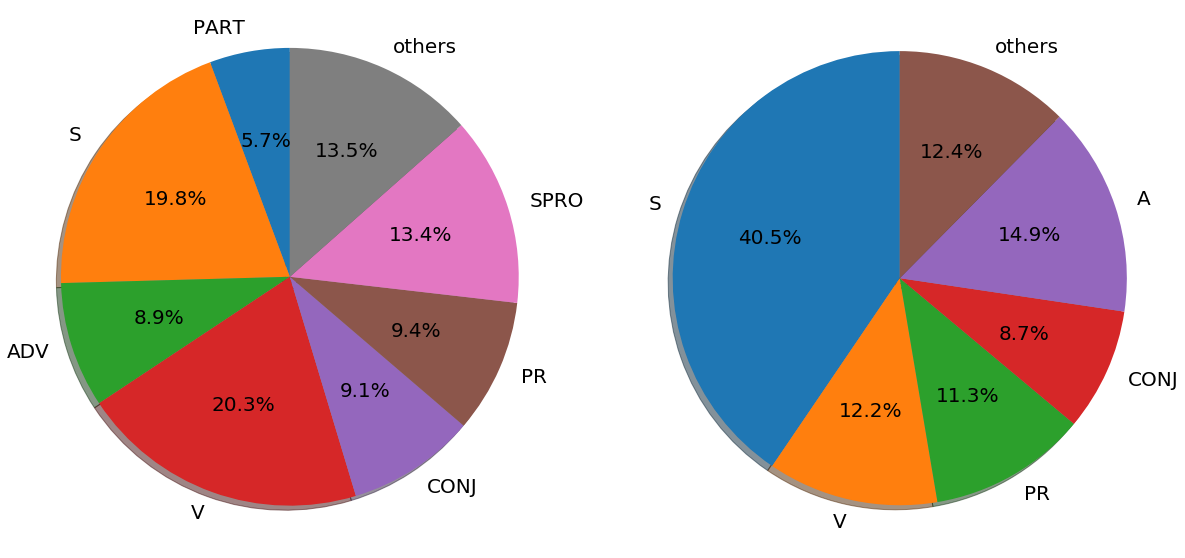
\includegraphics[width=\textwidth]{images/02.png}
\caption{Проценты частей речи, присутствующих в текстах}
\label{image:1}
\end{figure}

На рис. \ref{image:1} слева расположена диаграмма литературного текста, а справа -- научного. Можно заметить обилие частей речи, но довольно большой процент занимают служебные слова и союзы. Поэтому рассмотрим проценты частей речи текстов с исключенными стоп-словами.

\begin{figure}[h!]
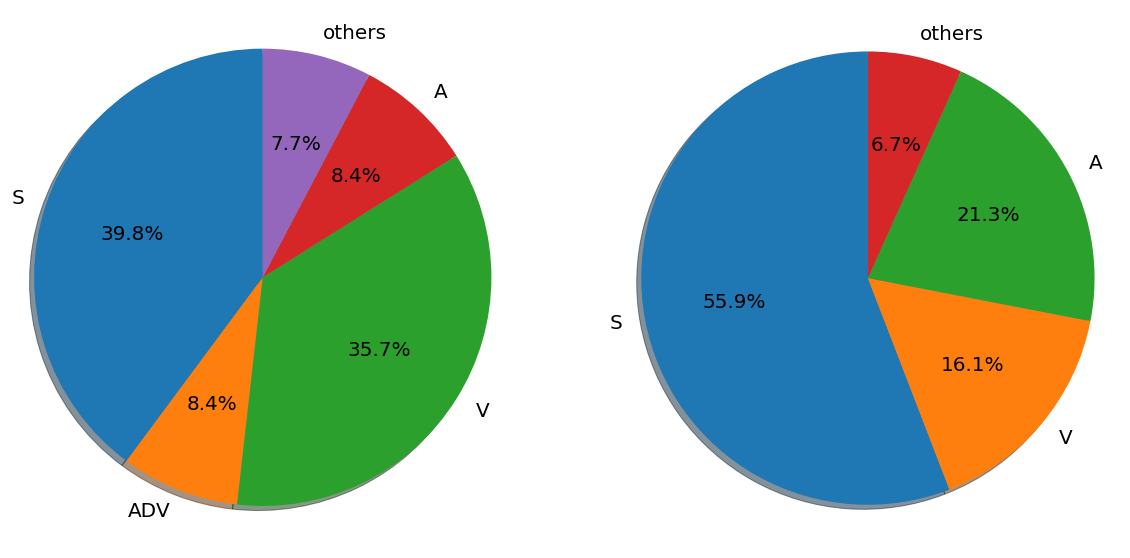
\includegraphics[width=\textwidth]{images/03.png}
\caption{Проценты частей речи, присутствующих в текстах (без стоп-слов)}
\label{image:2}
\end{figure}

На рис. \ref{image:2} хорошо видно то, что в литературном тексте (левая диаграмма) процент глаголов значительно больше чем в научном (правая диаграмма). Возможно так вышло из-за того, что в литературных текстах описывается много действий персонажей. В то же время в научном тексте гораздо больший процент существительных и прилагательных. Подобное преобладание существительны и прилагательных возможно исходит из того, что в научных текстах используется множество терминов, которые состоят из существительных или пар прилагательное-существительное.

\textit{Замечание.} MyStem умеет снимать омонимию по частям речи, но не всегда однозначно определяет все морфологические данные. К примеру он может предположить, что существительное может стоять в именительном или винительном падеже и вывести оба варианта.

\begin{table}[h!]
\centering
\begin{tabular}{ |p{3cm}||p{2cm}|p{2cm}|p{2cm}|p{2cm}| }
 \hline
 Падеж& Лит. &Науч. &Лит. отн. &Науч. отн.\\
 \hline
 им & 189 & 479 & 0.35 & 0.29\\
 вин & 143 & 453 & 0.26 & 0.27\\
 род & 91 & 373 & 0.17 & 0.23 \\
 пр & 44 & 146 & 0.08 & 0.09 \\
 дат & 40 & 111 & 0.07 & 0.07 \\
 твор & 29 & 90 & 0.05 & 0.05 \\
 местн & 7 & - & 0.01 & - \\
 парт & 3 & - & 0.01 & - \\
 \hline
\end{tabular}
\caption{Таблица частот падежей среди существительных}
\label{table:4}
\end{table}

В таблице \ref{table:4} можно сразу заметить то, что в научном тексте не используются местный падеж и партитив. В остальном все примерно одинаково с литературным текстом. Самые частотные падежи в обоих текстах именительный, винительный и родительный.

\begin{table}[h!]
\centering
\begin{tabular}{ |p{3cm}||p{2cm}|p{2cm}|p{2cm}|p{2cm}| }
 \hline
 Падеж& Лит. &Науч. &Лит. отн. &Науч. отн.\\
 \hline
 им & 38 & 105 & 0.32 & 0.17\\
 вин & 29 & 196 & 0.24 & 0.32\\
 род & 14 & 119 & 0.12 & 0.19 \\
 пр & 14 & 89 & 0.12 & 0.14 \\
 твор & 13 & 56 & 0.11 & 0.09 \\
 дат & 12 & 53 & 0.10 & 0.09 \\
 \hline
\end{tabular}
\caption{Таблица частот падежей среди прилагательных}
\label{table:5}
\end{table}

По таблице \ref{table:5} видно, что список самых частотных падежей у прилагательных совпадает с существительными. Можно отметить то, что в научном тексте прилагательные в именительном падеже встречаются не так часто, как в винительном и родительном.

\begin{table}[h!]
\centering
\begin{tabular}{ |p{7cm}||p{2cm}|p{2cm}| }
 \hline
 Характеристика& Лит. &Науч. \\
 \hline
 Число уникальных лемм & 623 & 700 \\
 Число уникальных лемм сущ. & 189 & 321 \\
 Число уникальных лемм прил. & 199 & 221 \\
 Число уникальных лемм гл. & 294 & 181 \\
 Число уникальных лемм нар. & 105 & 53 \\
 Коэффициент лексического богатства & 0.3923 & 0.3682 \\
 \hline
 Число незнакомых слов & 7 & 45 \\
 \hline
\end{tabular}
\caption{Таблица лексических характеристик текстов}
\label{table:6}
\end{table}

\begin{table}[h!]
\centering
\begin{tabular}{ |p{7cm}||p{2cm}|p{2cm}| }
 \hline
 Характеристика& Лит. &Науч. \\
 \hline
 Число уникальных лемм & 493 & 622 \\
 Число уникальных лемм сущ. & 172 & 303 \\
 Число уникальных лемм прил. & 123 & 188 \\
 Число уникальных лемм гл. & 243 & 158 \\
 Число уникальных лемм нар. & 57 & 34 \\
 Коэффициент лексического богатства & 0.6547 & 0.4701 \\
 \hline
\end{tabular}
\caption{Таблица лексических характеристик текстов без стоп-слов}
\label{table:7}
\end{table}

Из таблицы \ref{table:6} видно, что в научном тексте больше незнакомых слов, но скорее всего если взять другой литературный текст (например в жанре фентези, где присутствует великое множество выдуманных слов), то в литературном тексте незнакомых слов будет больше.

Сравнивая таблицы \ref{table:6} и \ref{table:7}, можно заметить то, что лексическое богатство обоих текстов примерно одинаковое до тех пор пока в них присутствуют стоп-слова. Без стоп-слов лексическое богатство литературного текста оказывается больше. Скорее всего это связано с тем, что научные тексты обычно пишут в рамках какой-то одной области и часто используют одни и те же термины.

\begin{table}[h!]
\centering
\begin{tabular}{ |p{3cm}||p{3cm}||p{3cm}|p{3cm}| }
 \hline
 Лит. слово& Отн. частота & Науч. слово & Отн. частота\\
 \hline
 алиса & 0.0412 & слово & 0.0340 \\
 мышь & 0.0252 & текст & 0.0234 \\
 подумать & 0.0120 & образ & 0.0144 \\
 кошка & 0.0093 & представлять & 0.0144\\
 прощать & 0.0066 & средство & 0.0113 \\
 \hline
\end{tabular}
\caption{Самые частотные слова обоих текстов без стоп-слов}
\label{table:8}
\end{table}

Из указанных в таблице \ref{table:8} самых частотных слов можно понять, что главными героями литературного текста являются Алиса и мышь и что научный рассказывает об исследовании связанном с представлением текста. Для большей наглядности можно взглянуть на рис. \ref{fig:sfig1} и \ref{fig:sfig2}, где изображены графики частот 20 самых частотных слов обоих текстов без стоп-слов.

\begin{figure}
\begin{subfigure}{\textwidth}
\centering
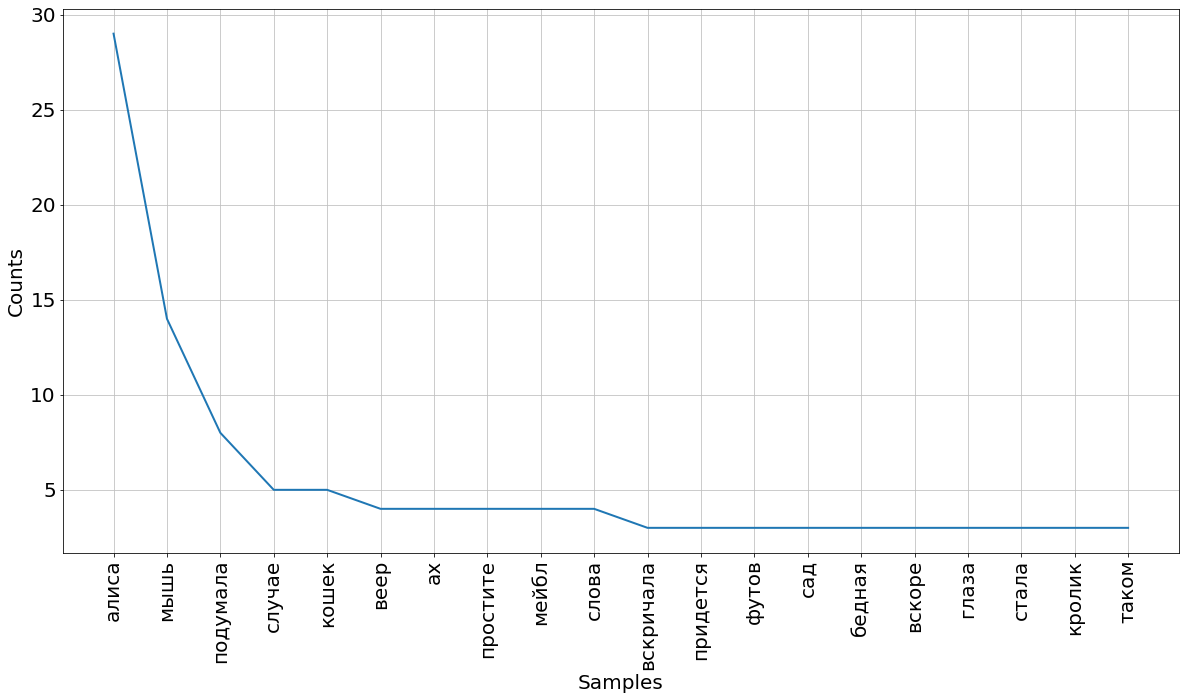
\includegraphics[width=\linewidth]{images/01-3}
\caption{Литературный текст без стоп-слов}
\label{fig:sfig1}
\end{subfigure}
\begin{subfigure}{\textwidth}
\centering
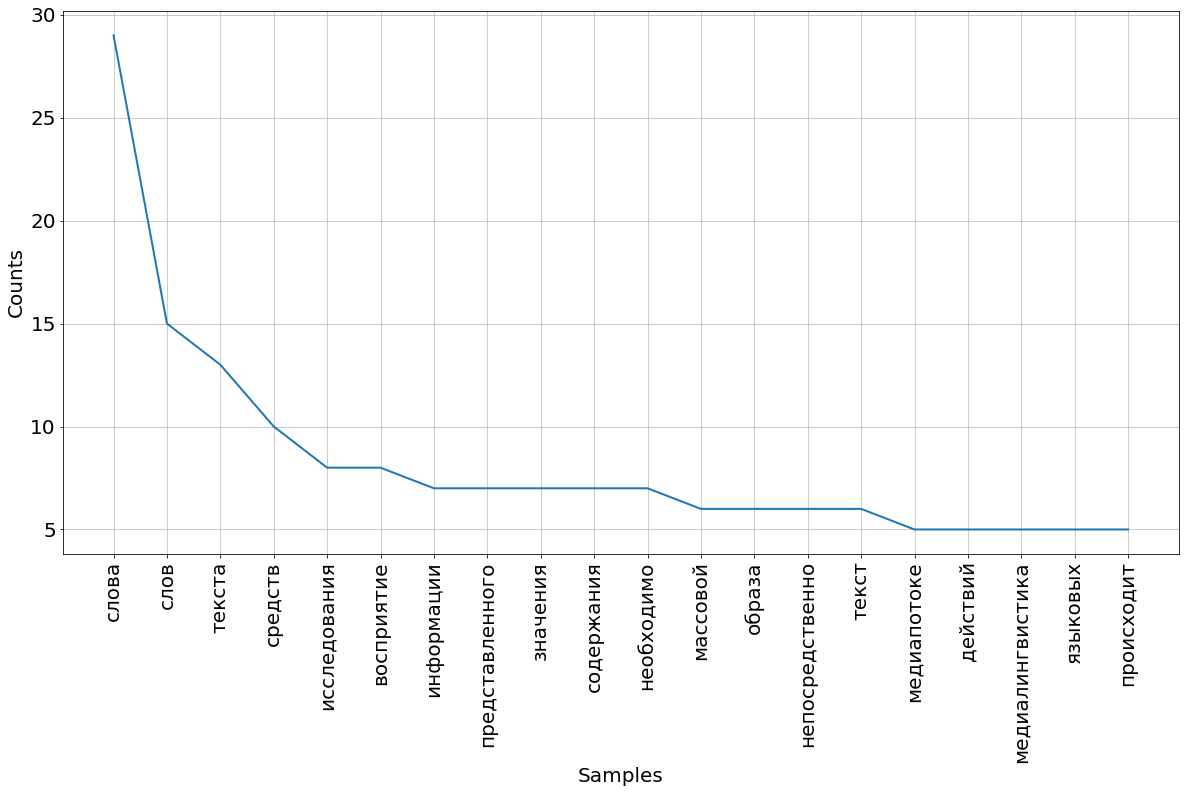
\includegraphics[width=\linewidth]{images/01-4}
\caption{Научный текст без стоп-слов}
\label{fig:sfig2}
\end{subfigure}
\end{figure}

\subsection*{Заключение}

После лексико-статистического анализа литературного и научного текстов на русском языке можно сказать, что в текстах разных видов прозы наблюдаются разные распределения морфологических характеристик. Вполне вероятно, что можно использовать эти данные для автоматического определения типа текста (литературный, научный и возможно др.).


\end{document}